\section{Introduction: Perfect Subsets of the Real Line}

Descriptive set theory nowadays is understood as the study of definable subsets of Polish Spaces. Many of its problems and techniques arose out of efforts to answer basic questions about the real numbers. A prominent example is the \textit{Continuum Hypothesis} ($\CH$):

\begin{framed}
\textbf{Continuum Hypothesis (Cantor, 1890s)}\\
If $A \subseteq \Real$ is uncountable, then there exists a bijection between $A$ and $\Real$. That is, is every uncountable subset of $\Real$ is of the same cardinality as $\Real$.
\end{framed}

Early approaches tried to show that $\CH$ holds for a number of sets with an easy topological structure.

For closed sets, the situation is less clear. Given a set $A \subseteq \Real$, we call $x \in \Real$ a \textbf{limit point} of $A$ if

\begin{equation}
\forall \epsilon > 0 \: \exists z \in A \: [z \neq x \: \& \: z \in U_\eps(x)],
\end{equation}

where $U_\eps(x)$ denotes the standard $\eps$-neighborhood of $x$ in $\Real$

\begin{definition}\label{def-perfect}A non-empty set $P \subseteq \Real$ is \textbf{perfect} if it is closed and every point of $P$ is a limit point.

\end{definition}In other words, a perfect set is a closed set that has no isolated points. We can also deduce that for a perfect set $P$, every neighborhood of a point $p \in P$ contains infinitely many points from $P$.

\begin{figure}[!htbp]
\centering
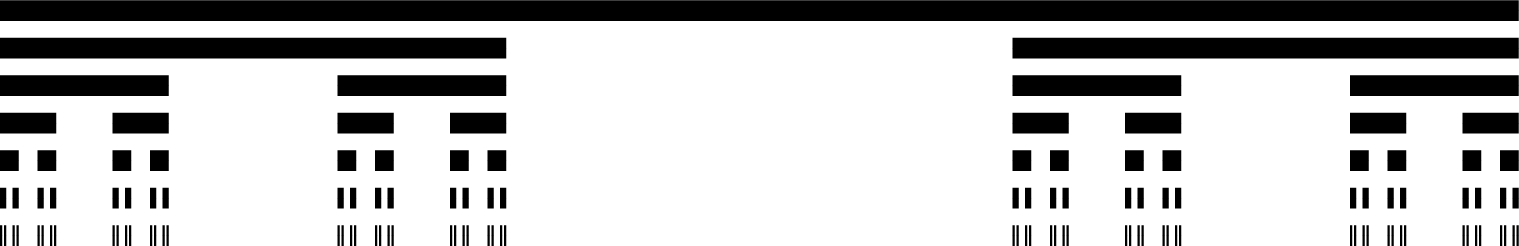
\includegraphics[width=0.7\linewidth]{files/Cantor_set-7f15a3eb647d25cf38092c5cd78d7432.png}
\caption*{Cantor set}
\end{figure}

Obviously, $\Real$ itself is perfect, as is any closed interval in $\Real$. There are totally disconnected perfect sets, such as the \textbf{middle-third Cantor set} in $[0,1]$

\begin{framed}
\textbf{Theorem (Cantor, 1884)}\\
A perfect subset of $\Real$ has the same cardinality as $\Real$.
\end{framed}

\begin{framed}
\textbf{Hint}\\
\begin{itemize}
\item Argue it suffices to construct an injection from $\Cant$ (the set of all infinite binary sequences) into the perfect set.
\item Start with any point $x$ in the perfect set and open neighborhood $U_\eps(x)$. Use the perfect set property to find two points $x_0, x_1$ distinct from $x$ and each other in $U_\eps(x)$.
\item These points will `guide' the mapping: All sequences in $\Cant$ starting with 0 will be mapped to a point close to $x_0$, while all sequences starting with 1 will be a mapped to a point close to $x_1$.
\item Now iterate with $x_0$ and $x_1$ in place of $x$.
\end{itemize}
\end{framed}

\begin{proof}Let $P \subseteq \Real$ be perfect. We construct an injection from the set $\Cant$ of all infinite binary sequences into $P$. An infinite binary sequence $\xi = \xi_0 \xi_1 \xi_2 \dots$ can be identified with a real number $\in [0,1]$ via the mapping

\begin{equation}
\xi \mapsto \sum_{i \geq 0} \xi_i 2^{-i-1}.
\end{equation}

Note that this mapping is onto. It follows that the cardinality of $P$ is at least as large as the cardinality of $[0,1]$. The \href{https://en.wikipedia.org/wiki/Schr\%C3\%B6der\%E2\%80\%93Bernstein\_theorem}{Schröder-Bernstein Theorem} (for a proof see e.g. \cite{jech2003a}) implies that $|P| = |\R|$.

To construct the desired injection, choose $x \in P$ and let $\eps_0 = 1 = 2^0$. Since $P$ is perfect, $P \cap U_{\eps_0}(x)$ is infinite. Let $x_0 \neq x_1$ be two points in $P \cap U_{\eps_0}(x)$, distinct from $x$. Let $\eps_1$ be such that $\eps_1 \leq 1/2$, $U_{\eps_1}(x_0), U_{\eps_1}(x_1) \subseteq U_{\eps_0}(x)$, and $\overline{U_{\eps_1}(x_0)} \cap \overline{U_{\eps_1}(x_1)} = \emptyset$, where $\overline{U}$ denotes the closure of $U$.

We can iterate this procedure recursively with smaller and smaller diameters, using the fact that $P$ is perfect. This gives rise to a so-called \textbf{Cantor scheme}, a family of open balls $(U_\sigma)$ satisfying certain \textit{nesting conditions}. Here the index $\sigma$ is a finite binary sequence, also called a \textit{string}. A Cantor scheme is defined by the following properties.

\begin{enumerate}
\item $\diam(U_\sigma) \leq 2^{ -|\sigma|}$, where $|\sigma|$ denotes the length of $\sigma$.
\item If $\tau$ is a proper extension of $\sigma$, then $U_\tau \subset U_\sigma$.
\item If $\tau$ and $\sigma$ are \textit{incompatible} (i.e. neither extends the other), then
\begin{equation*}
U_\tau \cap U_\sigma = \emptyset.
\end{equation*}

\item The center of each $U_\sigma$, call it $x_\sigma$, is in $P$.
\end{enumerate}

\begin{figure}[!htbp]
\centering
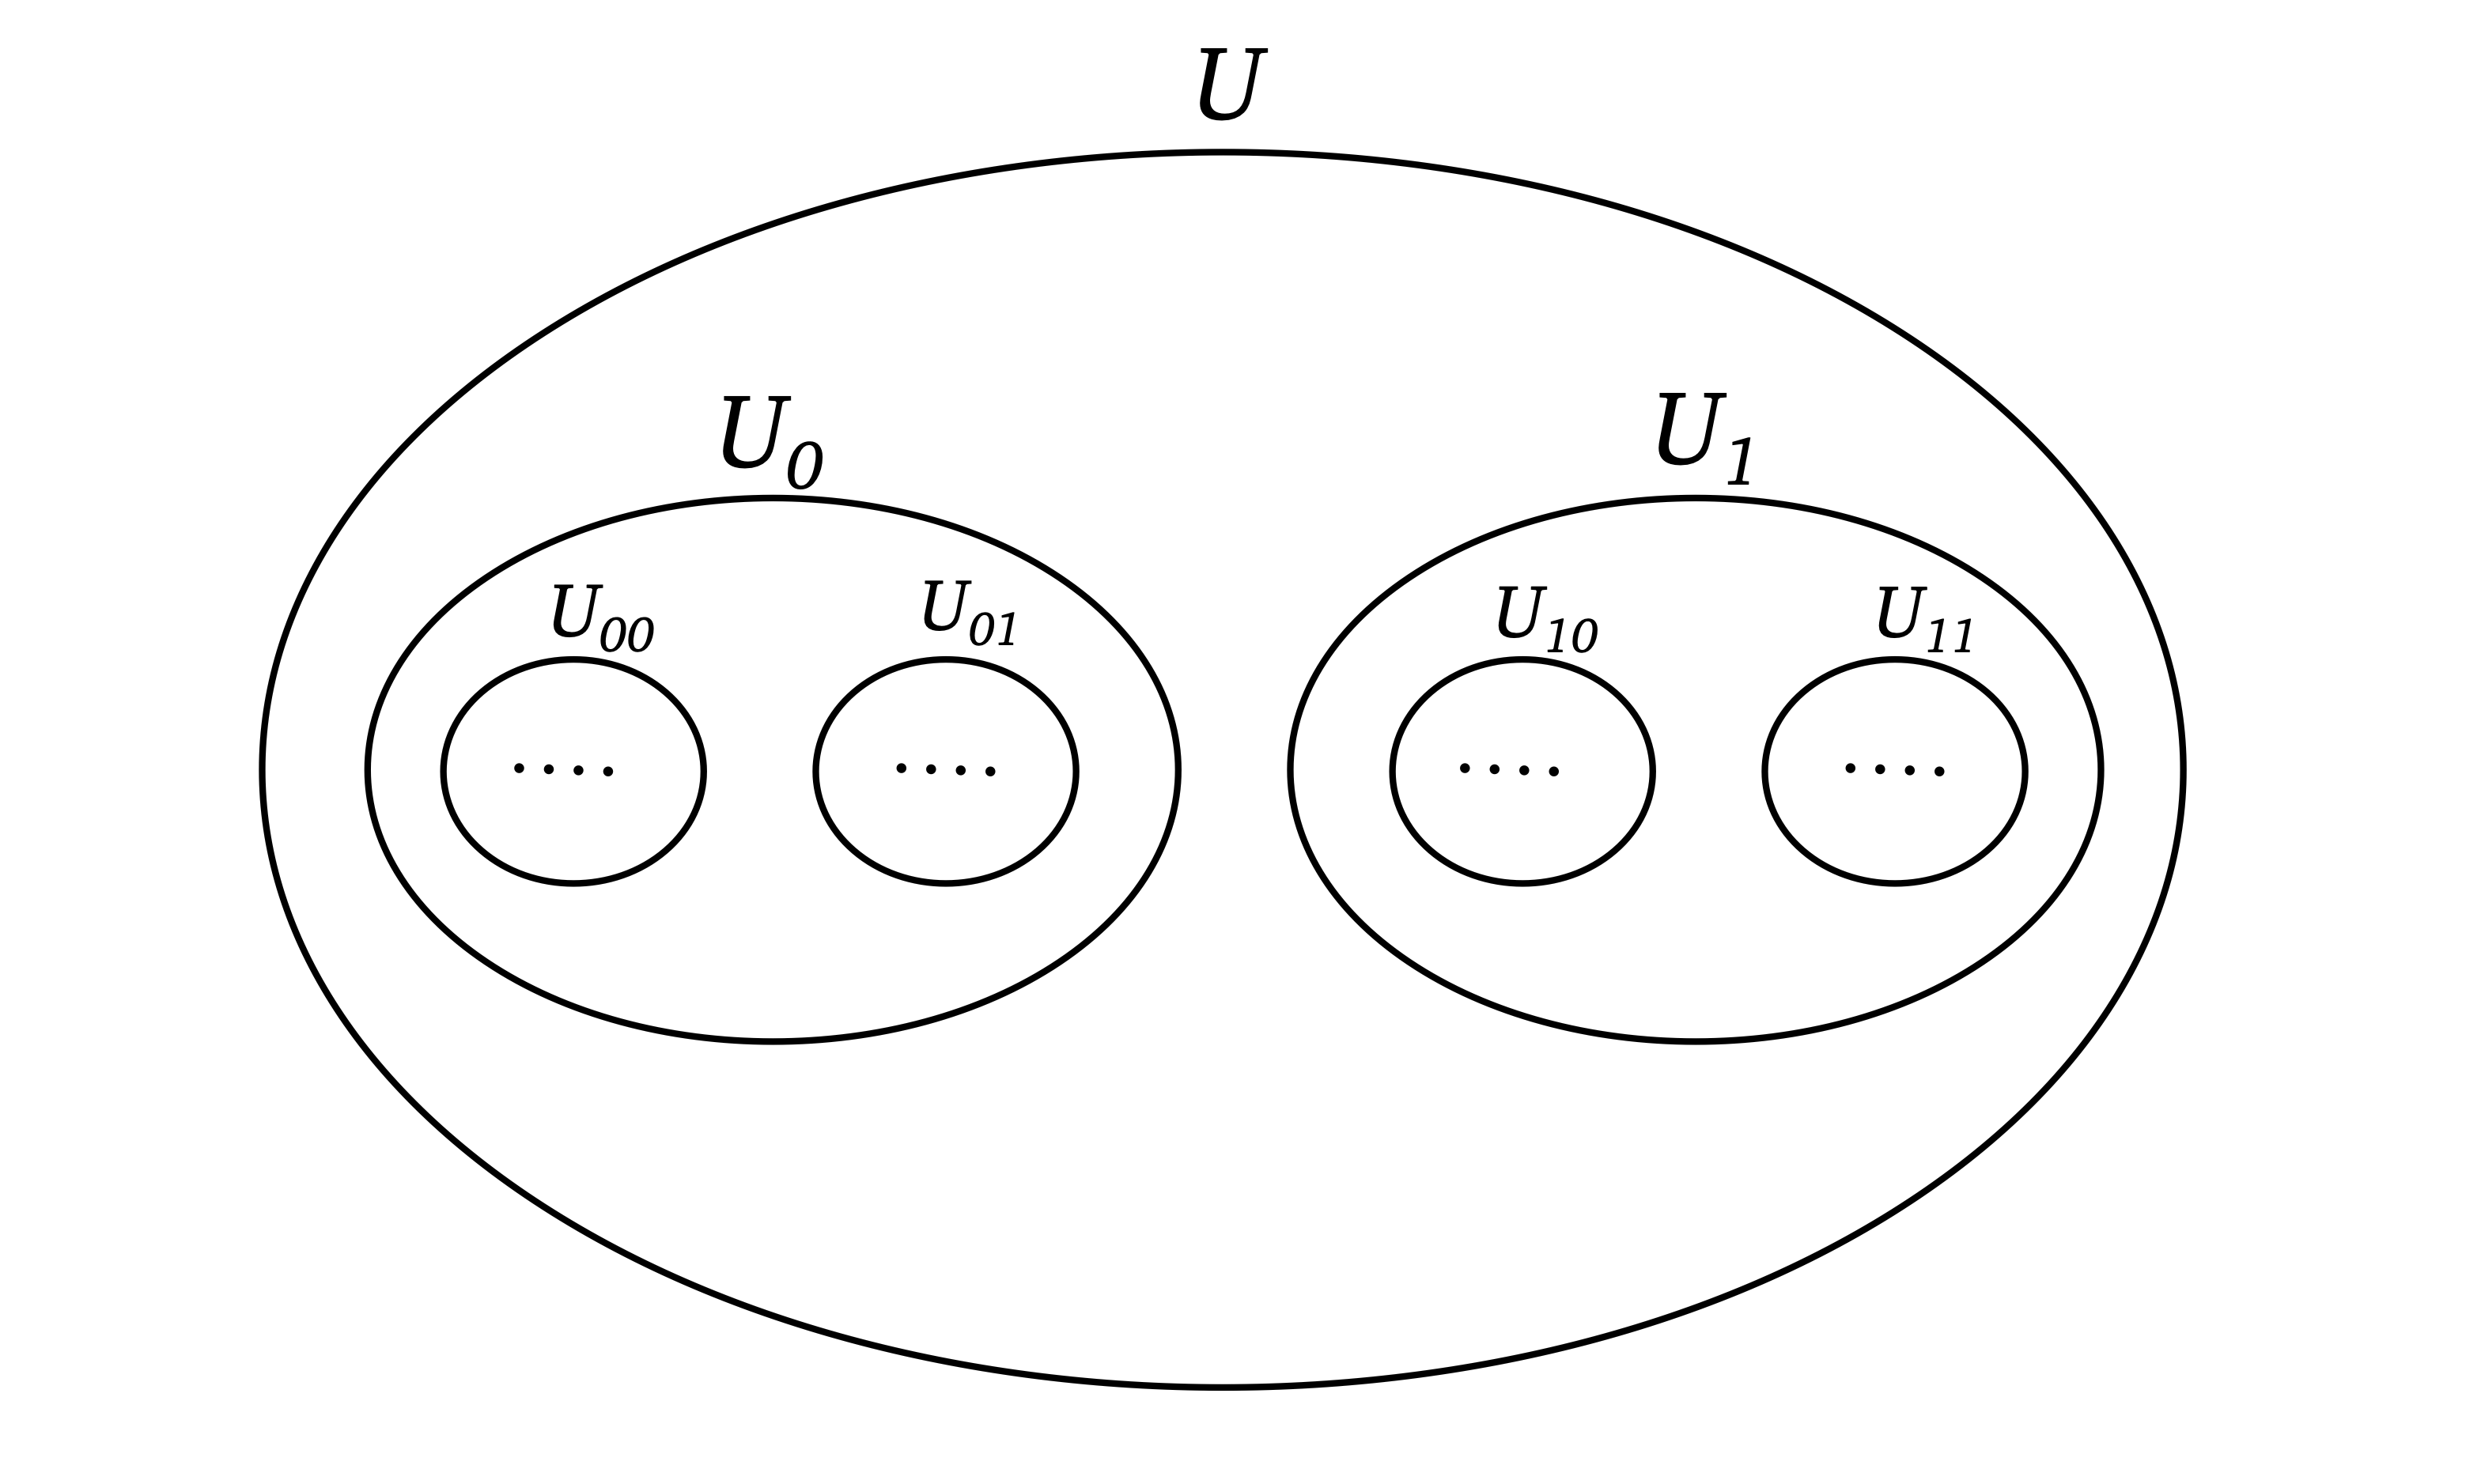
\includegraphics[width=0.7\linewidth]{files/Cantor_Scheme-0b52d5260abb5f7f4d0a22abe7957d4c.png}
\caption[]{Nested structure of a Cantor scheme}
\label{Cantor Scheme}
\end{figure}

Let $\xi$ be an infinite binary sequence. Given $n \geq 0$, we denote by $\xi\Rest{n}$ the string formed by the first $n$ bits of $\xi$, i.e.

\begin{equation}
\xi\Rest{n} = \xi_0 \xi_1 \dots \xi_{n-1}.
\end{equation}

The finite initial segments give rise to a sequence $x_{\xi\Rest{n}}$ of centers. By properties (1.) and (2.), this is a Cauchy sequence. By (4.), the sequence lies in $P$. Since $P$ is closed, the limit $x_\xi$ is in $P$. By (3.), the mapping $\xi \mapsto x_\xi$ is well-defined and injective.

\end{proof}Thus, to show that a set of reals has the same cardinality as $\R$, it suffices to show the set contains a perfect subset. The next theorem establishes that the Continuum Hypothesis holds for all closed subsets of $\R$.

\begin{framed}
\textbf{Cantor-Bendixson Theorem}\\
Every uncountable closed subset of $\Real$ contains a perfect subset.
\end{framed}

\begin{framed}
\textbf{Hint}\\
Consider the set of \textbf{condensation points}, i.e. the set of all points for which any open neighborhood has \textit{uncountable} intersection with the given closed set.
\end{framed}

\begin{proof}Let $C \subseteq \Real$ be uncountable and closed. We say $z \in \Real$ is a \textit{condensation point} of $C$ if

\begin{equation}
\forall \eps > 0 \:[ U_\eps(z) \cap C \text{ uncountable}].
\end{equation}

Let $D$ be the set of all condensation points of $C$. Note that $D \subseteq C$, since every condensation point is clearly a limit point and $C$ is closed.

Furthermore, we claim that $D$ is perfect. Clearly $D$ is closed. Suppose $z \in D$ and $\eps > 0$. Then $U_\eps(z) \cap C$ is uncountable. We would like to conclude that $U_\eps(z) \cap D$ is uncountable, too, since this would mean in particular that $U_\eps(z) \cap D$ is infinite. The conclusion holds if $C \setminus D$ is countable.

To show that $C\setminus D$ is countable, assume that $y \in C \setminus D$. Then, for some $\delta > 0$, $U_\delta(y) \cap C$ is countable. We can find and interval $I(y) \subseteq U_\delta(y)$ that contains $y$ and has rational endpoints. There are at most countably many intervals with rational endpoints and hence for each $y \in C \setminus D$ there are at most countably many choices for $I(y)$. Thus, we have

\begin{equation}
C\setminus D \subseteq \bigcup_{y \in C \setminus D} I_y \cap C.
\end{equation}

The right hand side is a countable union of countable sets, hence countable.

\end{proof}We will later encounter an alternative (more constructive) proof that gives additional information about the complexity of the closed set $C$. For now we conclude with the fact we were aiming to prove in this lecture.

\begin{corollary}Every closed subset of $\Real$ is either countable or of the cardinality of the continuum.

\end{corollary}The results of this lecture give us a blueprint on how to verify the Continuum Hypothesis for a given family $\mathcal{F}$ of sets (of reals):

A family $\mathcal{F}$ of sets (of reals) has the \textbf{perfect set property} if every set in $\mathcal{F}$ is either countable or has a perfect subset.

\begin{framed}
\textbf{Question}\\
Which families of sets have the perfect set property?
\end{framed}